

% debut explication aprroche aleatoire sans remise avec cout unitaire 
Nous supposons que $p=0.5$ c'est-\`a-dire qu'il y'a autant de cases {\em fausses n\'egatives} que de cases {\em fausses positives} dans la matrice $M_{k,p}$.
\newline
Nous repr\'esentons les distributions des distances de correction et de Hamming, la fonction de repartition de la corr\'elation entre ces distances  et la fonction cumulative de la distance de Hamming. 
La distribution des distances de correction indique la proportion de graphes $LG_{k,p,\alpha}$ qui ont le m\^eme ensemble d'ar\^etes que les graphes $G_{k,p,\alpha}$. En ce qui concerne la distribution des distances de Hamming, elle indique  la proportion de graphes $LG_{k,p,\alpha}$ qui ont le m\^eme ensemble d'ar\^etes que les graphes $LG$.
La corr\'elation entre les distances de correction et de Hamming, not\'ee {\em correlation\_DC\_DH}, est calcul\'ee avec la formule \ref{correlation_correction_hamming}. Sa fonction de repartition $F_k(x)$ indique le nombre de corr\'elations inf\'erieures \`a une valeur de corr\'elation $x$ donn\'ee.
Quant \`a la fonction cumulative de la distance de Hamming, elle montre l'\'evolution du nombre de cases modifi\'ees de la matrice $M'_{k,p}$ en fonction du nombre de line-graphes  construites $LG$.
\newline
%\vspace{-0.5cm}
% -------------------- figure simulation_distanceMoyenDLDH_k_0_aleatoire_p_05 ------------------------
\begin{figure}[htb!] 
\centering
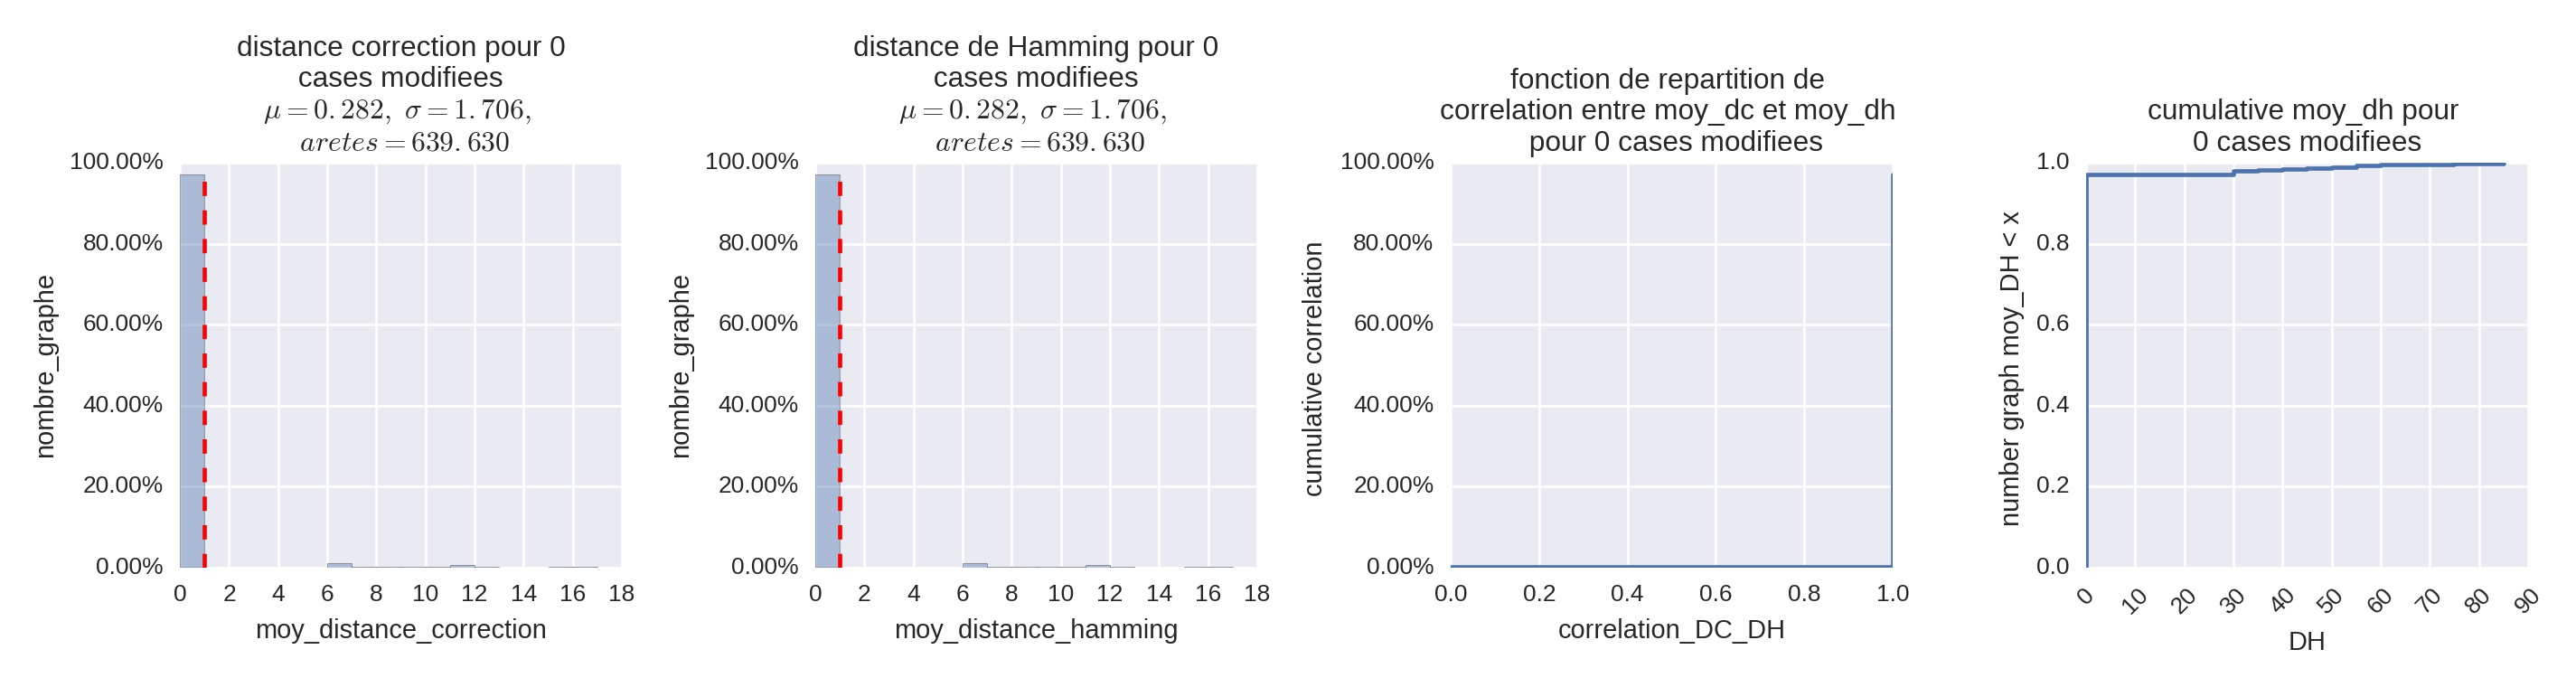
\includegraphics[width=500pt,height=160pt]{simulation_distanceMoyenDLDH_k_0_aleatoire_p_05.jpeg}
\caption{ Approche de correction al\'eatoire sans remise \`a co\^ut unitaire pour $k =0 $ case modifi\'ee. La premi\`ere colonne repr\'esente la distribution des distances correction $moy\_DC_{0,0.5}$. La seconde colonne est la distribution des distances de Hamming $moy\_DH_{0,0.5}$. La troisi\`eme colonne  est la fonction de repartition de la corr\'elation entre les distances de correction et de Hamming avec en abscisse la corr\'elation entre ces distances (correlation\_DC\_DH).  La quatri\`eme colonne est la fonction cumulative des distances de Hamming.}
\label{sansremise_unitaire_distanceMoyenDCDH_k_0_aleatoire_p_05} 
\end{figure}
\FloatBarrier
% -------------------- figure simulation_distanceMoyenDLDH_k_0_aleatoire_p_05 -----------------------

Les figures \ref{sansremise_unitaire_distanceMoyenDCDH_k_0_aleatoire_p_05} et \ref{sansremise_unitaire_distanceMoyenDCDH_k_1_2_5_9_aleatoire_p_05} pr\'esentent les courbes respectives pour $k=0$ et $k \in \{1,2,5,9\}$ cases modifi\'ees. 
La colonne $1$ indique la distribution des distances de correction, la colonne $2$ est la colonne de la distribution des distances de Hamming, la colonne $3$ est associ\'ee \`a la fonction de repartition de la corr\'elation entre les distances de correction et de Hamming avec en abscisse la corr\'elation entre ces distances ({\em correlation\_DC\_DH)}. 
Et la colonne $4$ est celle de la fonction cumulative des distances de Hamming.
Dans les colonnes $1$ et $2$, les distributions se divisent en deux zones: 
\begin{itemize}
\item Zone {\em gauche} ou {\em am\'eliorante} : elle correspond aux batonnets de l'intervalle $[0,k]$. Cet intervalle  am\'eliore l'ensemble $E'_{k,p,\alpha}$ des ar\^etes du graphe $LG_{k,p,\alpha}$ pour que $E'_{k,p,\alpha}$ soit identique \`a l'ensemble $E_{LG}$ des ar\^etes du graphe $LG$. Si $moy\_DH_{k,p} \rightarrow 0$ alors $LG_{k,p,\alpha}$ est tr\`es proche de $LG$. Si $moy\_DH_{k,p} \rightarrow k$ alors les matrices des graphes $LG_{k,p,\alpha}$ et $LG$ diff\`erent de $k$ cases et ces cases sont les $k$ cases modifi\'ees dans $LG$.
\item Zone {\em droite} ou {\em d\'egradante} : elle correspond aux batonnets de l'intervalle $]k, +\infty[$. Cet intervalle d\'eteriore  l'ensemble $E'_{k,p,\alpha}$ des ar\^etes du graphe $LG_{k,p,\alpha}$. Ainsi, le line-graphe $LG_{k,p,\alpha}$ s'\'eloigne de $LG$ quand $moy\_DH_{k,p} \rightarrow +\infty$.
\end{itemize}
Ces deux zones sont s\'epar\'ees par une droite en pointill\'ee d'\'equation $y = k$.  Cette droite d\'esigne le nombre de cases modifi\'ees dans le line-graphe $LG$.
\newline

Pour $k=0$ case modifi\'ee, nous v\'erifions que nos algorithmes sont coh\'erents c'est-\`a-dire que la phase de correction est inutile. En effet, nous avons $100\%$ de graphes $G_{k,p,\alpha}, LG_{k,p,\alpha}, LG$ qui ont les m\^emes ensembles d'ar\^etes et cela implique que $moy\_DH_{0,0.5} = moy\_DC_{0,0.5} = 0$. D'o\`u le seul batonnet dans les colonnes $1$ et $2$. Par ailleurs, la fonction de repartition de la corr\'elation et la fonction cumulative des distances de Hamming sont d\'efinies par les \'equations \ref{eqCorrelMoyDCDH} (a) et (b)  respectivement.
\begin{equation}
\label{eqCorrelMoyDCDH}
F_k(x_1) = \left\{
	\begin{aligned}
	0 \hspace{1 em} si \hspace{1 em} x_1 < 1 \\
	100  \hspace{1 em}  si  \hspace{1 em}  x_1 = 1
	\end{aligned}
	\right.(a)
	\\~~~~~~~
	y_{cumulDH}^{0}(x) = 1  \hspace{1 em}  si  \hspace{1 em}   x \in \N (b)
\end{equation}
%\begin{equation}
%\label{eqCumulMoyDH}
%y_{cumulDH}^{0}(x) = 1  \hspace{1 em}  si  \hspace{1 em}   x \in \N
%\end{equation}
avec $x_1$ la corr\'elation entre les distances et $x$ le nombre d'ar\^etes modifi\'ees.
Les valeurs des distances de Hamming sont \'egales \`a $0$ donc sa fonction cumulative $y_{cumulDH}^{k}$ vaut $1$. 
L'\'equation  \ref{eqCorrelMoyDCDH}(a) s'interpr\`ete comme suit : $F_k(x) = 100\%$ des line-graphes ont leurs distances de correction et de Hamming correl\'ees ($x = 1$).
\newline

% k = {1,2}
Pour $k \in \{1,2\}$, le pic des histogrammes se localise dans la zone {\em am\'eliorante} des colonnes $1$ et $2$ de la figure \ref{sansremise_unitaire_distanceMoyenDCDH_k_1_2_5_9_aleatoire_p_05} et son pourcentage est sup\'erieur \`a $50\%$. 
Les autres batonnets sont dans la zone {\em d\'egradante} et leur pic a un pourcentage inf\'erieur \`a $10\%$ en moyenne. 
Dans la colonne $1$ de la figure \ref{sansremise_unitaire_distanceMoyenDCDH_k_1_2_5_9_aleatoire_p_05}, le pic correspond aux $k$ cases modifi\'ees du graphe $G_{k,p,\alpha}$ et son pourcentage est identique \`a celui du pic de la colonne $2$. 
Le pic de la colonne $2$ correspond \`a $moy\_DH_{k,0.5} = 0$ et signifie que  $LG$ et $LG_{k,p,\alpha}$ ont le m\^eme ensemble d'ar\^etes. Ainsi, les $k \le 2$ cases modifi\'ees sont supprim\'ees de la matrice $M'_{k,p,\alpha}$ lorsque $moy\_DC_{k,0.5} \le k$.
Cependant, les distances de correction et de Hamming ont approximativement les m\^emes valeurs lorsque $moy\_DC_{k,0.5} > k$ ($moy\_DC_{k,0.5}$ est dans la partie {\em d\'egradante} de la figure \ref{sansremise_unitaire_distanceMoyenDCDH_k_1_2_5_9_aleatoire_p_05}). 
Cela s'explique par le fait que les distances $moy\_DC_{k,0.5}$ et $moy\_DH_{k,0.5}$ sont corr\'el\'ees. Nous d\'etaillons la notion de corr\'elation de distances dans la section \ref{relationMoyDHmoyDC}.
% ---- a ajouter dans la partie correlation
%En effet, la colonne $3$ de la figure \ref{sansremise_unitaire_distanceMoyenDLDH_k_1_2_5_9_aleatoire_p_05} d\'esigne les corr\'elations entre ces distances. Pour une corr\'elation $x > 0.3$, $F_k(x) > 60\%$ et  pour $x \le 0.3$, $F_k(x) < 5\%$. Or $F_k(x)\rightarrow 0\%$ signifie que $moy\_DL$ est \'egale \`a $k$ ($moy\_DL = k$) et $moy\_DH$ tend vers $k$ ($moy\_DH \rightarrow k$). Donc $F_k(x) < 5\%$ implique que $moy\_DL = k$ et $moy\_DH \approx k$.
Ainsi, les distances de correction et de Hamming sont corr\'el\'ees dans $\eta_k = 5\%$ des line-graphes $LG_{k,p,\alpha}$ et le line-graphe $LG_{k,p,\alpha}$ devient le line-graphe initial $LG$ si nous corrigons les $DC$ cases modifi\'ees du graphe $LG_{k,p,\alpha}$. 
La variable $\eta_k$ est la proportion de line-graphes dont les distances de correction et de Hamming sont fortement corr\'el\'ees.
\newline

% ------------------- figure permut_distanceMoyenDLDH_k_1_2_5_9_aleatoire_p_05 ------------------
\begin{figure}[htb!] 
%\centering
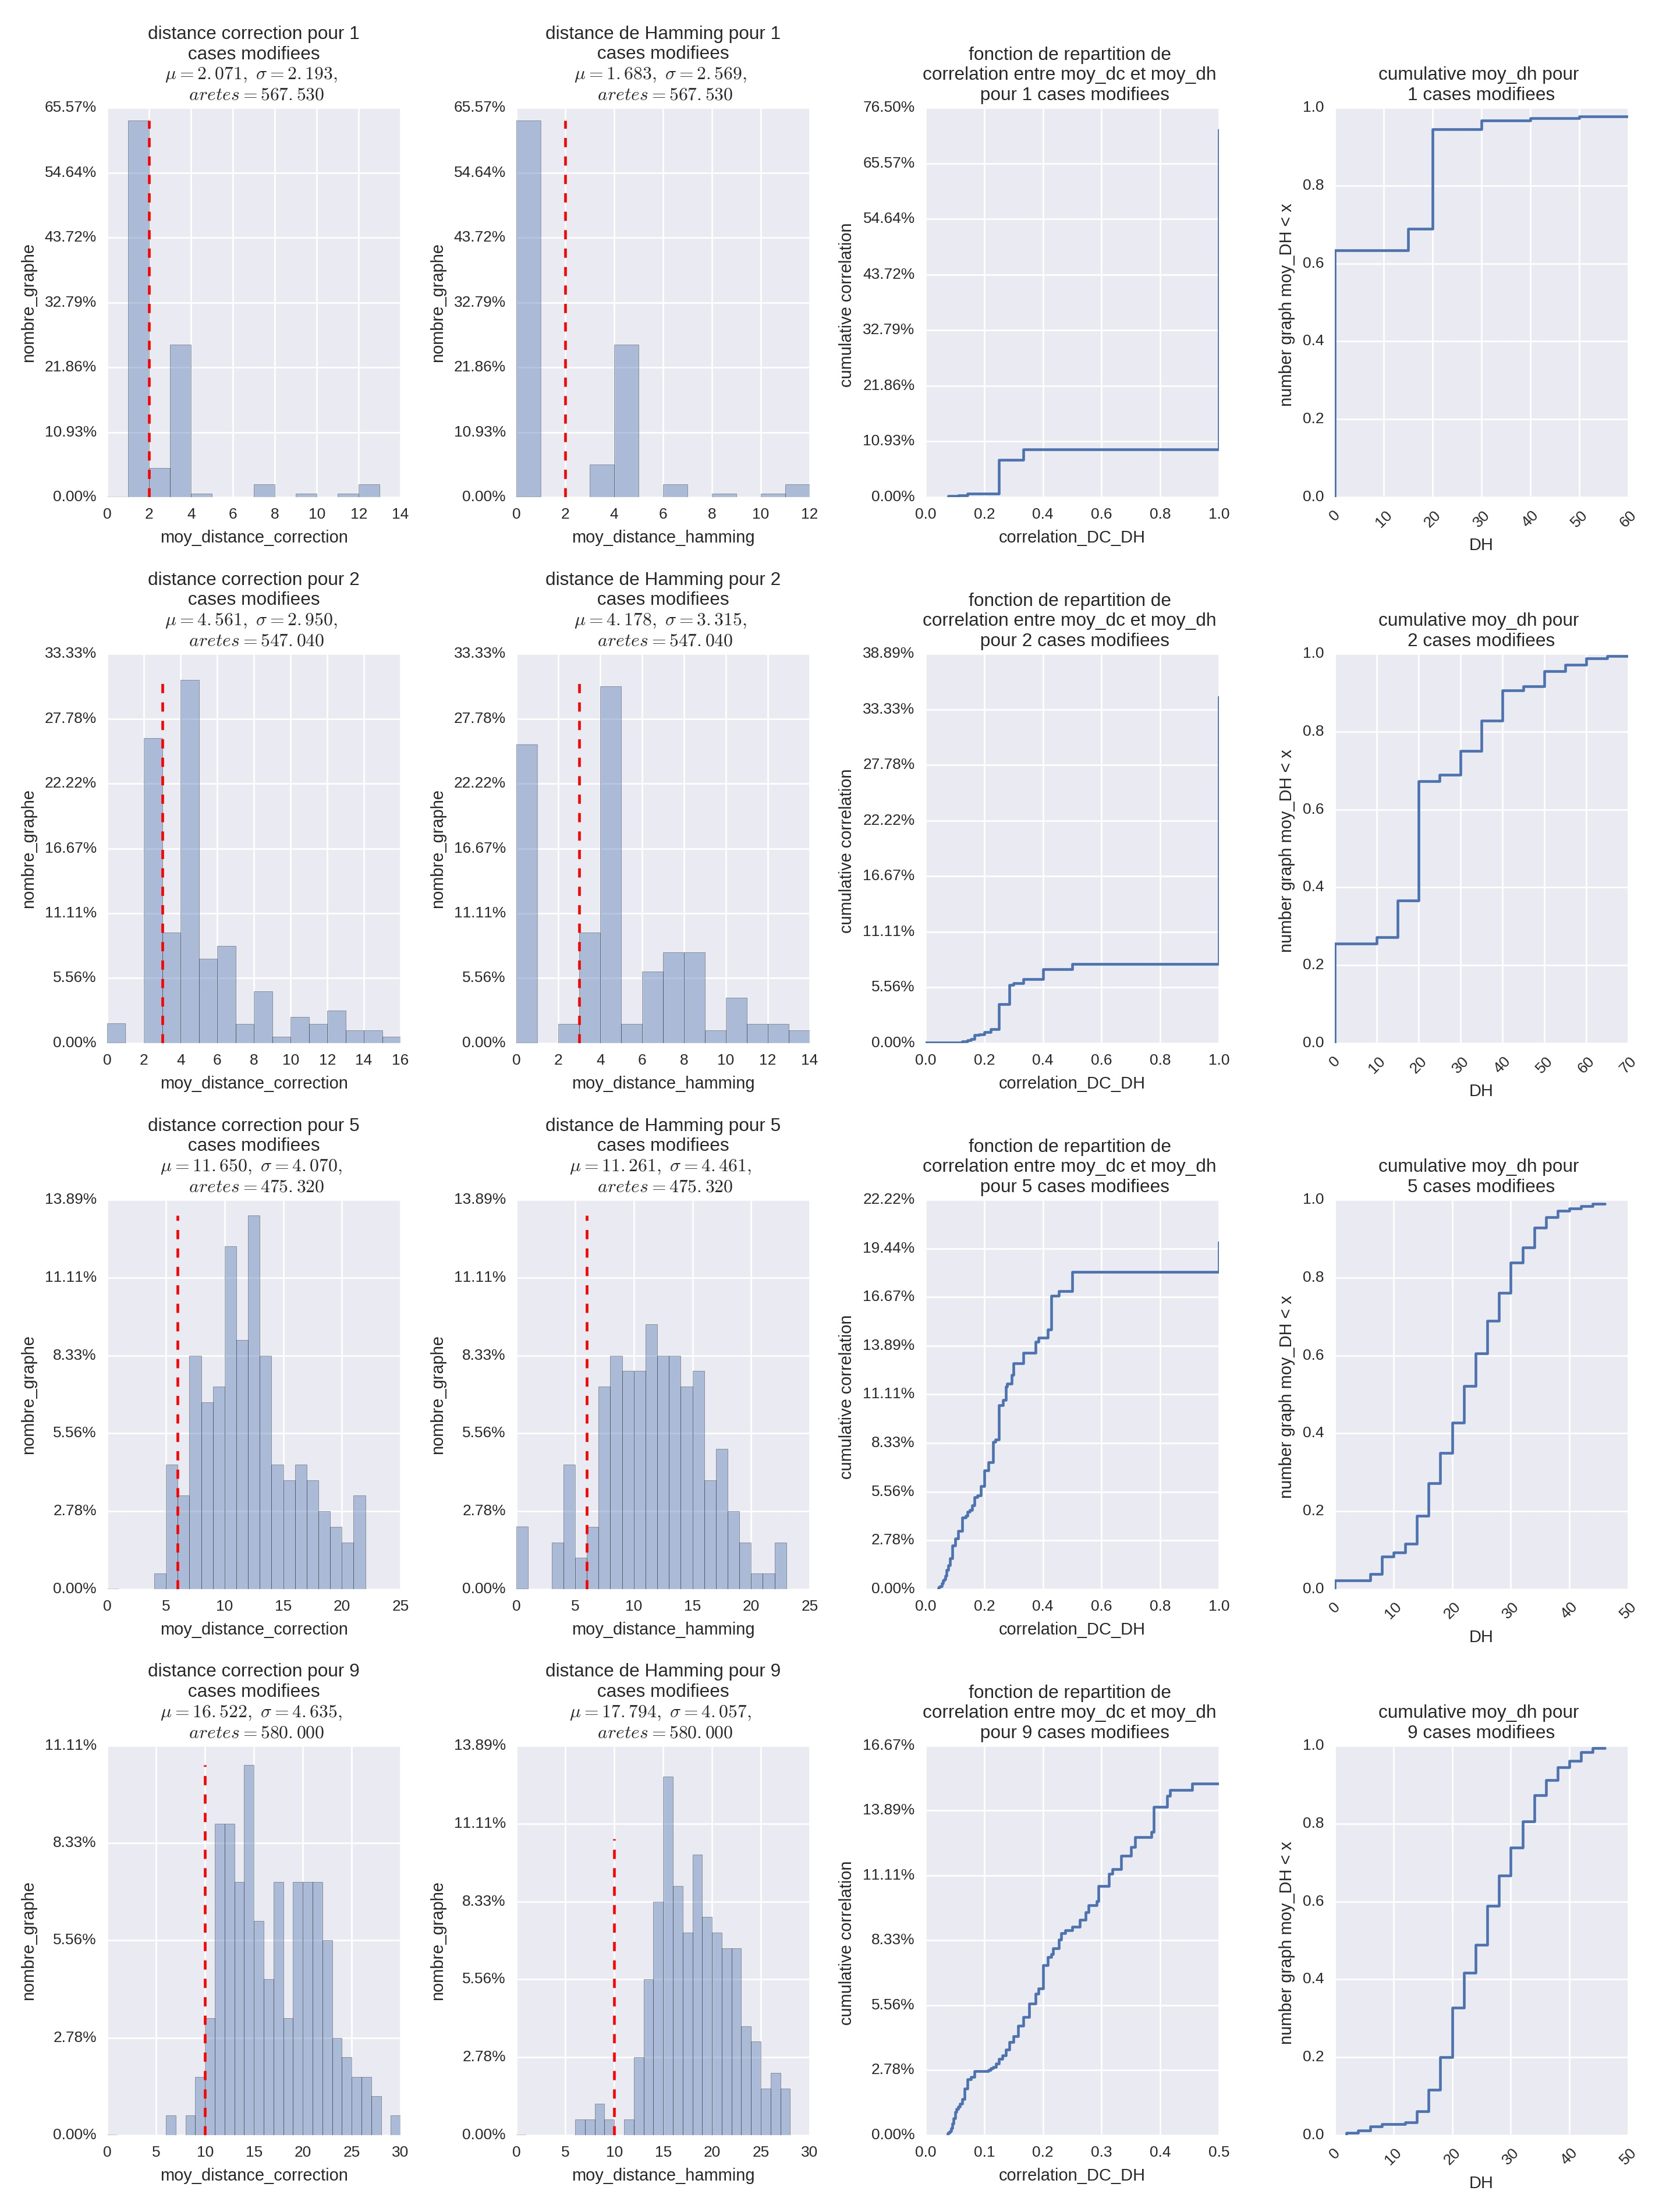
\includegraphics[width=550pt,height=570pt]{permut_distanceMoyenDLDH_k_1_2_5_9_aleatoire_p_05.jpeg}
\caption{ Approche de correction al\'eatoire sans remise \`a co\^ut unitaire pour $k =\{1,2,5,9\} $ cases modifi\'ees :
 La premi\`ere colonne repr\'esente la distribution des distances de correction $moy\_DC_{k,0.5}$. La seconde colonne est la distribution des distances de Hamming $moy\_DH_{k,0.5}$. 
 La troisi\`eme colonne  est la fonction de repartition de la corr\'elation entre les distances de correction et de Hamming avec en abscisse la corr\'elation entre ces distances (correlation\_DC\_DH).  
 La quatri\`eme colonne est la fonction cumulative des distances de Hamming. 
 La premi\`ere ligne est associ\'ee \`a $k=1$ case modifi\'ee, 
 la seconde ligne \`a $k=2$ cases modifi\'ees, 
 la troisi\`eme ligne \`a $5$ cases modifi\'ees et enfin 
 la derni\`ere \`a $9$ cases modifi\'ees.
 }
\label{sansremise_unitaire_distanceMoyenDCDH_k_1_2_5_9_aleatoire_p_05} 
\end{figure}
\FloatBarrier
% ----------------- figure permut_distanceMoyenDLDH_k_1_2_5_9_aleatoire_p_05 ---------------------

% k = 5
Pour $k = 5$, le pic se trouve toujours dans la zone {\em am\'eliorante} des colonnes $1$ et $2$ de la figure \ref{sansremise_unitaire_distanceMoyenDCDH_k_1_2_5_9_aleatoire_p_05} mais son pourcentage baisse significativement \`a $15.69\%$ (voir la ligne $3$). 
Le nombre de  line-graphes dans la zone {\em d\'egradante} dans les colonnes $1$ et $2$ augmente tout comme les distances de correction et de Hamming qui atteignent  jusqu'\`a $45$ ar\^etes.
La variable $\eta_k$ est \'egale \`a  $18.38\%$ de line-graphes $LG_{k,p,\alpha}$ (voir ligne $3$ de la colonne $3$ de la figure \ref{sansremise_unitaire_distanceMoyenDCDH_k_1_2_5_9_aleatoire_p_05}).
Cette augmentation provient de la baisse du pourcentage du pic de la zone {\em am\'eliorante} au profit de la zone {\em d\'egradante} et la plupart des graphes appartenant \`a cette zone ont leurs distances de correction et de Hamming corr\'el\'ees.
Les $15.69\%$  de line-graphes $LG_{k,p,\alpha}$ identiques \`a $LG$ s'expliquent par le type de cases modifi\'ees et l'emplacement des ar\^etes dans le graphe $LG$.  En effet, ces cases modifi\'ees sont des {\em fausses n\'egatives} et ces ar\^etes supprim\'ees n'appartiennent pas \`a des cliques voisines. Toutefois, quelque soit le type de cases modifi\'ees, notre couple d'algorithmes ajoutent beaucoup d'ar\^etes pour obtenir le line-graphe $LG_{k,p,\alpha}$ lorsque les cases sont reparties avec $p = 0.5$. Par exemple, nous avons constat\'e, en moyenne, $10$ \`a $20$ ar\^etes diff\'erentes pour $k=5$ cases modifi\'ees dans nos exp\'erimentations. 
Par ailleurs, nous remarquons qu'il existe des graphes dans lesquels la distance de correction est inf\'erieure \`a $k$. Tel est le cas pour $k = 5$ ou nous avons $moy\_DC_{k,0.5} = 3$ et $nombre\_graphe = 0.14\%$ dans la colonne $1$  de la figure \ref{sansremise_unitaire_distanceMoyenDCDH_k_1_2_5_9_aleatoire_p_05}.
En effet, les cases modifi\'ees sont des cases {\em fausses n\'egatives}. Ces ar\^etes supprim\'ees de $LG$ appartiennent \`a la m\^eme clique et certaines ar\^etes sont ajout\'ees de telle sorte que la clique se partitionne en deux cliques.   
%les aretes appartiennent a une meme cliques  de tel sorte qu'il ajoute certains aretes qui sindent la clique en deux cliques
%1) lalgo ajoute des aretes
%2) ces aretes  appartiennent a la meme clique et elles sont ajoutes de tel sorte que il forme deux cliques
\newline 

% k = 9
Enfin, pour $k=9$, la distribution des valeurs de distances est dans la zone {\em d\'egradante} et le pic est \`a $moy\_DC_{k,0.5} = 23$ cases modifi\'ees avec un pourcentage de $6\%$ line-graphes.  
En comparant les pourcentages des distances $moy\_DC_{k,0.5}$ et $moy\_DH_{k,0.5}$, nous constatons qu'ils ne sont pas identiques comme pour $k \le 5$. En effet, certaines cases modifi\'ees ne sont pas corrig\'ees car l'algorithme de correction modifie \'enorm\'ement de cases qui sont diff\'erentes des $k$ cases et ce taux croit quand  $moy\_DC_{k,0.5}$ est \'elev\'e. 
Le taux de cases corrig\'ees est de $53.38\%$ en moyenne.
La variable $\eta_k$ passe \`a $22\%$ de line-graphes $LG_{k,p,\alpha}$ parce que la correction a modifi\'ee des cases diff\'erentes des $k$ cases. Cependant les distances de correction et de Hamming restent toujours corr\'el\'ees et $3\%$ line-graphes $LG_{k,p,\alpha}$ ont le m\^eme ensemble d'ar\^etes que $LG$ (voir ligne $4$ de la colonne $3$ de la figure \ref{sansremise_unitaire_distanceMoyenDCDH_k_1_2_5_9_aleatoire_p_05}).
C'est pourquoi, les courbes de  $F_k(x)$ et $y_{cumulDH}^{k}$ ont cette forme enrob\'ee proche de la fonction  sigmoide de param\^etre $\lambda \le -15$. Pour rappel, nous pr\'ecisons que ces courbes  tendent vers la fonction suivante $f_{\lambda}(x) = \frac{1}{1+e^{\lambda * (x-0.5)}}$.
\newline
Les  cases modifi\'ees $k \in \{1,\cdots,9\}$ sont pr\'esent\'ees dans les figures 
 \ref{sansremise_unitaire_distanceMoyenDCDH_k_1_5_aleatoire_p_05} et  
\ref{sansremise_unitaire_distanceMoyenDCDH_k_6_9_aleatoire_p_05} de l'annexe \ref{annexe_distribution_0_9}.
\newline
% fin explication mode aleatoire sans remise avec cout unitaire 

L'approche de correction $(2c)$ nous montre que les distances de correction et de Hamming se d\'egradent quand le nombre $k$ de cases modifi\'ees augmentent. En fait, pour $k \le 5$, le nombre de line-graphes $LG_{k,p,\alpha}$ identiques \`a $LG$ est sup\'erieur \`a $nombre\_graphe = 25\%$ avec des distances de correction $moy\_DC_{k,0.5} = k$. Pour des distances $moy\_DC_{k,0.5} = 2 \times k$, les  $k$ cases modifi\'ees sont corrig\'ees. 
Des cases \'erron\'ees sont ajout\'ees pendant l'ex\'ecution de l'algorithme de correction mais elles sont peu nombreuses. Nous pouvons consid\'erer ces cases comme la pr\'ecision de notre algorithme  car ces cases indiquent le nombre de cases \`a modifier pour obtenir $LG$. Ainsi la distance de correction est major\'ee par le nombre de cases $k$ modifi\'ees.
Cependant, au d\'el\`a de $k > 5$,  la distance de correction $moy\_DC_{k,0.5}$ double et moins de $50\%$ des $k$ cases sont corrig\'ees. Les cases \'erron\'ees ajout\'ees proviennent de l'ajout et la suppression d'ar\^etes dans le line-graphe $LG'_{k,p,\alpha}$ \'etant donn\'ee que la fonction de co\^ut est {\em unitaire}. La distance de correction est major\'ee par $2 \times k$ en moyenne.
\newline

{\bf Conclusion} : l'approche de correction {\em al\'eatoire sans remise} $(2c)$ propose des line-graphes $LG_{k,p}$  identiques \`a $LG$ quand $k \le 5$. Dans ce cas, le probl\`eme {\em Proxi-Line} est trait\'e car la distance line est major\'ee par $k$. 
Toutefois, le nombre de cases \`a corriger apr\`es l'ex\'ecution de notre couple d'algorithmes est faible lorsque la distance de correction est inf\'erieure au double de $k$ ($moy\_DC_{k,0.5} = 2 \times k$) avec $k>5$. Cela conduit \`a majorer la distance line par le double des cases \'erron\'ees.
En outre, pour $k>5$, le pourcentage  $\eta_k$ de corr\'elation entre $moy\_DC_{k,0.5}$ et $moy\_DH_{k,0.5}$ croit. Nous allons \'etudier l'\'evolution de $\eta_k$  dans le paragraphe \ref{relationMoyDHmoyDC} mais nous commencons par la comparaison des diff\'erentes approches de correction pour en d\'eduire celle qui minimise les distances de correction ou de Hamming.

